\documentclass[a4paper]{article}

%% Language and font encodings
\usepackage[english,italian]{babel}
\usepackage[utf8x]{inputenc}
\usepackage[T1]{fontenc}

%% Sets page size and margins
\usepackage[a4paper,top=3cm,bottom=2cm,left=3cm,right=3cm,marginparwidth=1.75cm]{geometry}

%% Useful packages
\usepackage{amsmath}
\usepackage{amsfonts}
\usepackage{bm}
\usepackage{graphicx}
\usepackage[colorinlistoftodos]{todonotes}
\usepackage[colorlinks=true, all colors=blue]{hyperref} %referenze linkate
\usepackage{booktabs}
\usepackage{siunitx}  %notaz. espon. con \num{} e unità di misura in SI con \si{}
\usepackage{xcolor}
\usepackage{colortbl}
\usepackage{bm}
\usepackage{caption} 
\usepackage{indentfirst}
\usepackage{physics} 
\usepackage{rotating}
\usepackage{tabularx}
\usepackage{url}
\usepackage{pst-plot}
\usepackage{comment} %per usare l'ambiente {comment}
\usepackage{float} 
\usepackage{subfig}
\usepackage[americanvoltages]{circuitikz} %per disegnare circuiti
\usepackage{tikz}
\usepackage{mathtools} %per allineare su più linee in ambiente {align} o {align*}
\usepackage{cancel}
\renewcommand{\CancelColor}{\color{lightgray}}
%\setlength{\parindent}{0cm}


\graphicspath{{Figure/}}
\captionsetup{format=hang,labelfont={sf,bf},font=small}
\captionsetup{tableposition=top,figureposition=bottom,font=small}
\captionsetup[table]{skip=8pt}
%Comando per l'unit\'a di misura A^1\2
\newcommand{\radamp}[0]{\ \text{A}^{1/2}}
\newcommand{\kz}{K^0}
\newcommand{\bkz}{\bar{K}^0}
\newcommand{\kzs}{\ket{K^0}}
\newcommand{\bkzs}{\ket{\bar{K}^0}}
%\renewcommand{\dag}[1]{{#1}^\dagger}


\title{Domanda SubNuc}
\author{Giorgio Palermo}




\begin{document}
\hypersetup{linkcolor = black}
\hypersetup{linkcolor = blue}

\begin{center}
    \textbf{MASTER'S DEGREE IN PHYSICS}
    
    Academic Year 2019-2020
    
    \medskip
    \textbf{Introduction to Many Body Theory}
\end{center}

\vspace{0.8cm}
Student: Giorgio Palermo

Student ID: 1238258

Date: May 15, 2020

\bigskip

\begin{center}
\textbf{HOMEWORK 3}
\end{center}


\section*{Exercise (a)}
The expressions for the diagrams presented in the image below are the following:
\begin{align*}
G^{(2a)}_{\alpha\beta}(x,y) = \int \dd{x_1}\dd{x_1'}\dd{x_2}\dd{x_2'} &G^0_{\alpha\lambda}(x,x_1)U(x1,x_1')_{\substack{\lambda\lambda'\\ \mu\mu'}}G^0_{\mu\mu'}(x_1,x_1')G^0_{\lambda'\nu}(x_1,x_2)\times \\
&\times U(x_2,x_2')_{\substack{\nu\nu'\\ \sigma\sigma'}}G^0_{\sigma\sigma'}(x_2,x_2') G^0_{\nu'\beta}(x_2,y)\\
G^{(2b)}_{\alpha\beta}(x,y) = \int \dd{x_1}\dd{x_2}\dd{x_3}\dd{x_4} &G^0_{\alpha\lambda}(x,x_1)U(x_1,x_2)_{\substack{\lambda\lambda'\\ \mu\mu'}} G^0_{\lambda'\mu'}(x_1,x_2) G^0_{\mu\nu}(x_2,x_3) \times \\
&\times U(x_3,x_4)_{\substack{\nu\nu'\\ \sigma\sigma'}}G^0_{\nu'\sigma'}(x_3,x_4)G^0_{\alpha\beta}(x,y)\\
G^{(2c)}_{\alpha\beta}(x,y) = \int \dd{x_1}\dd{x_2}\dd{x_3}\dd{x_3'} &G^0_{\alpha\lambda}(x,x_1) U(x_1,x_2)_{\substack{\lambda\lambda'\\ \mu\mu'}} G^0_{\lambda'\mu'}(x_1,x_2) G^0_{\mu\nu}(x_2,x_3)\times\\
&\times U(x_3,x_3')_{\substack{\nu\nu'\\\sigma\sigma'}} G^0_{\sigma\sigma'}(x_3,x_3') G^0_{\nu'\beta}(x_3,y)\\
G^{(2d)}_{\alpha\beta}(x,y) = \int \dd{x_1}\dd{x_2}\dd{x_3}\dd{x_3'} &G^0_{\alpha\nu'}(x,x_3) U(x_3,x_3')_{\substack{\nu'\nu\\ \sigma'\sigma}} G^0_{\sigma'\sigma}(x_3',x_3') G^0_{\nu\mu'}(x_3,x_2) \times \\
&\times U(x_2,x_1)_{\substack{\mu\mu' \\ \lambda'\lambda}}  G^0_{\mu\lambda'}(x_2,x_1) G^0_{\lambda\beta}(x_1,y)
\end{align*}


\begin{figure}[h]
\centering
\label{fig:diagabcd}
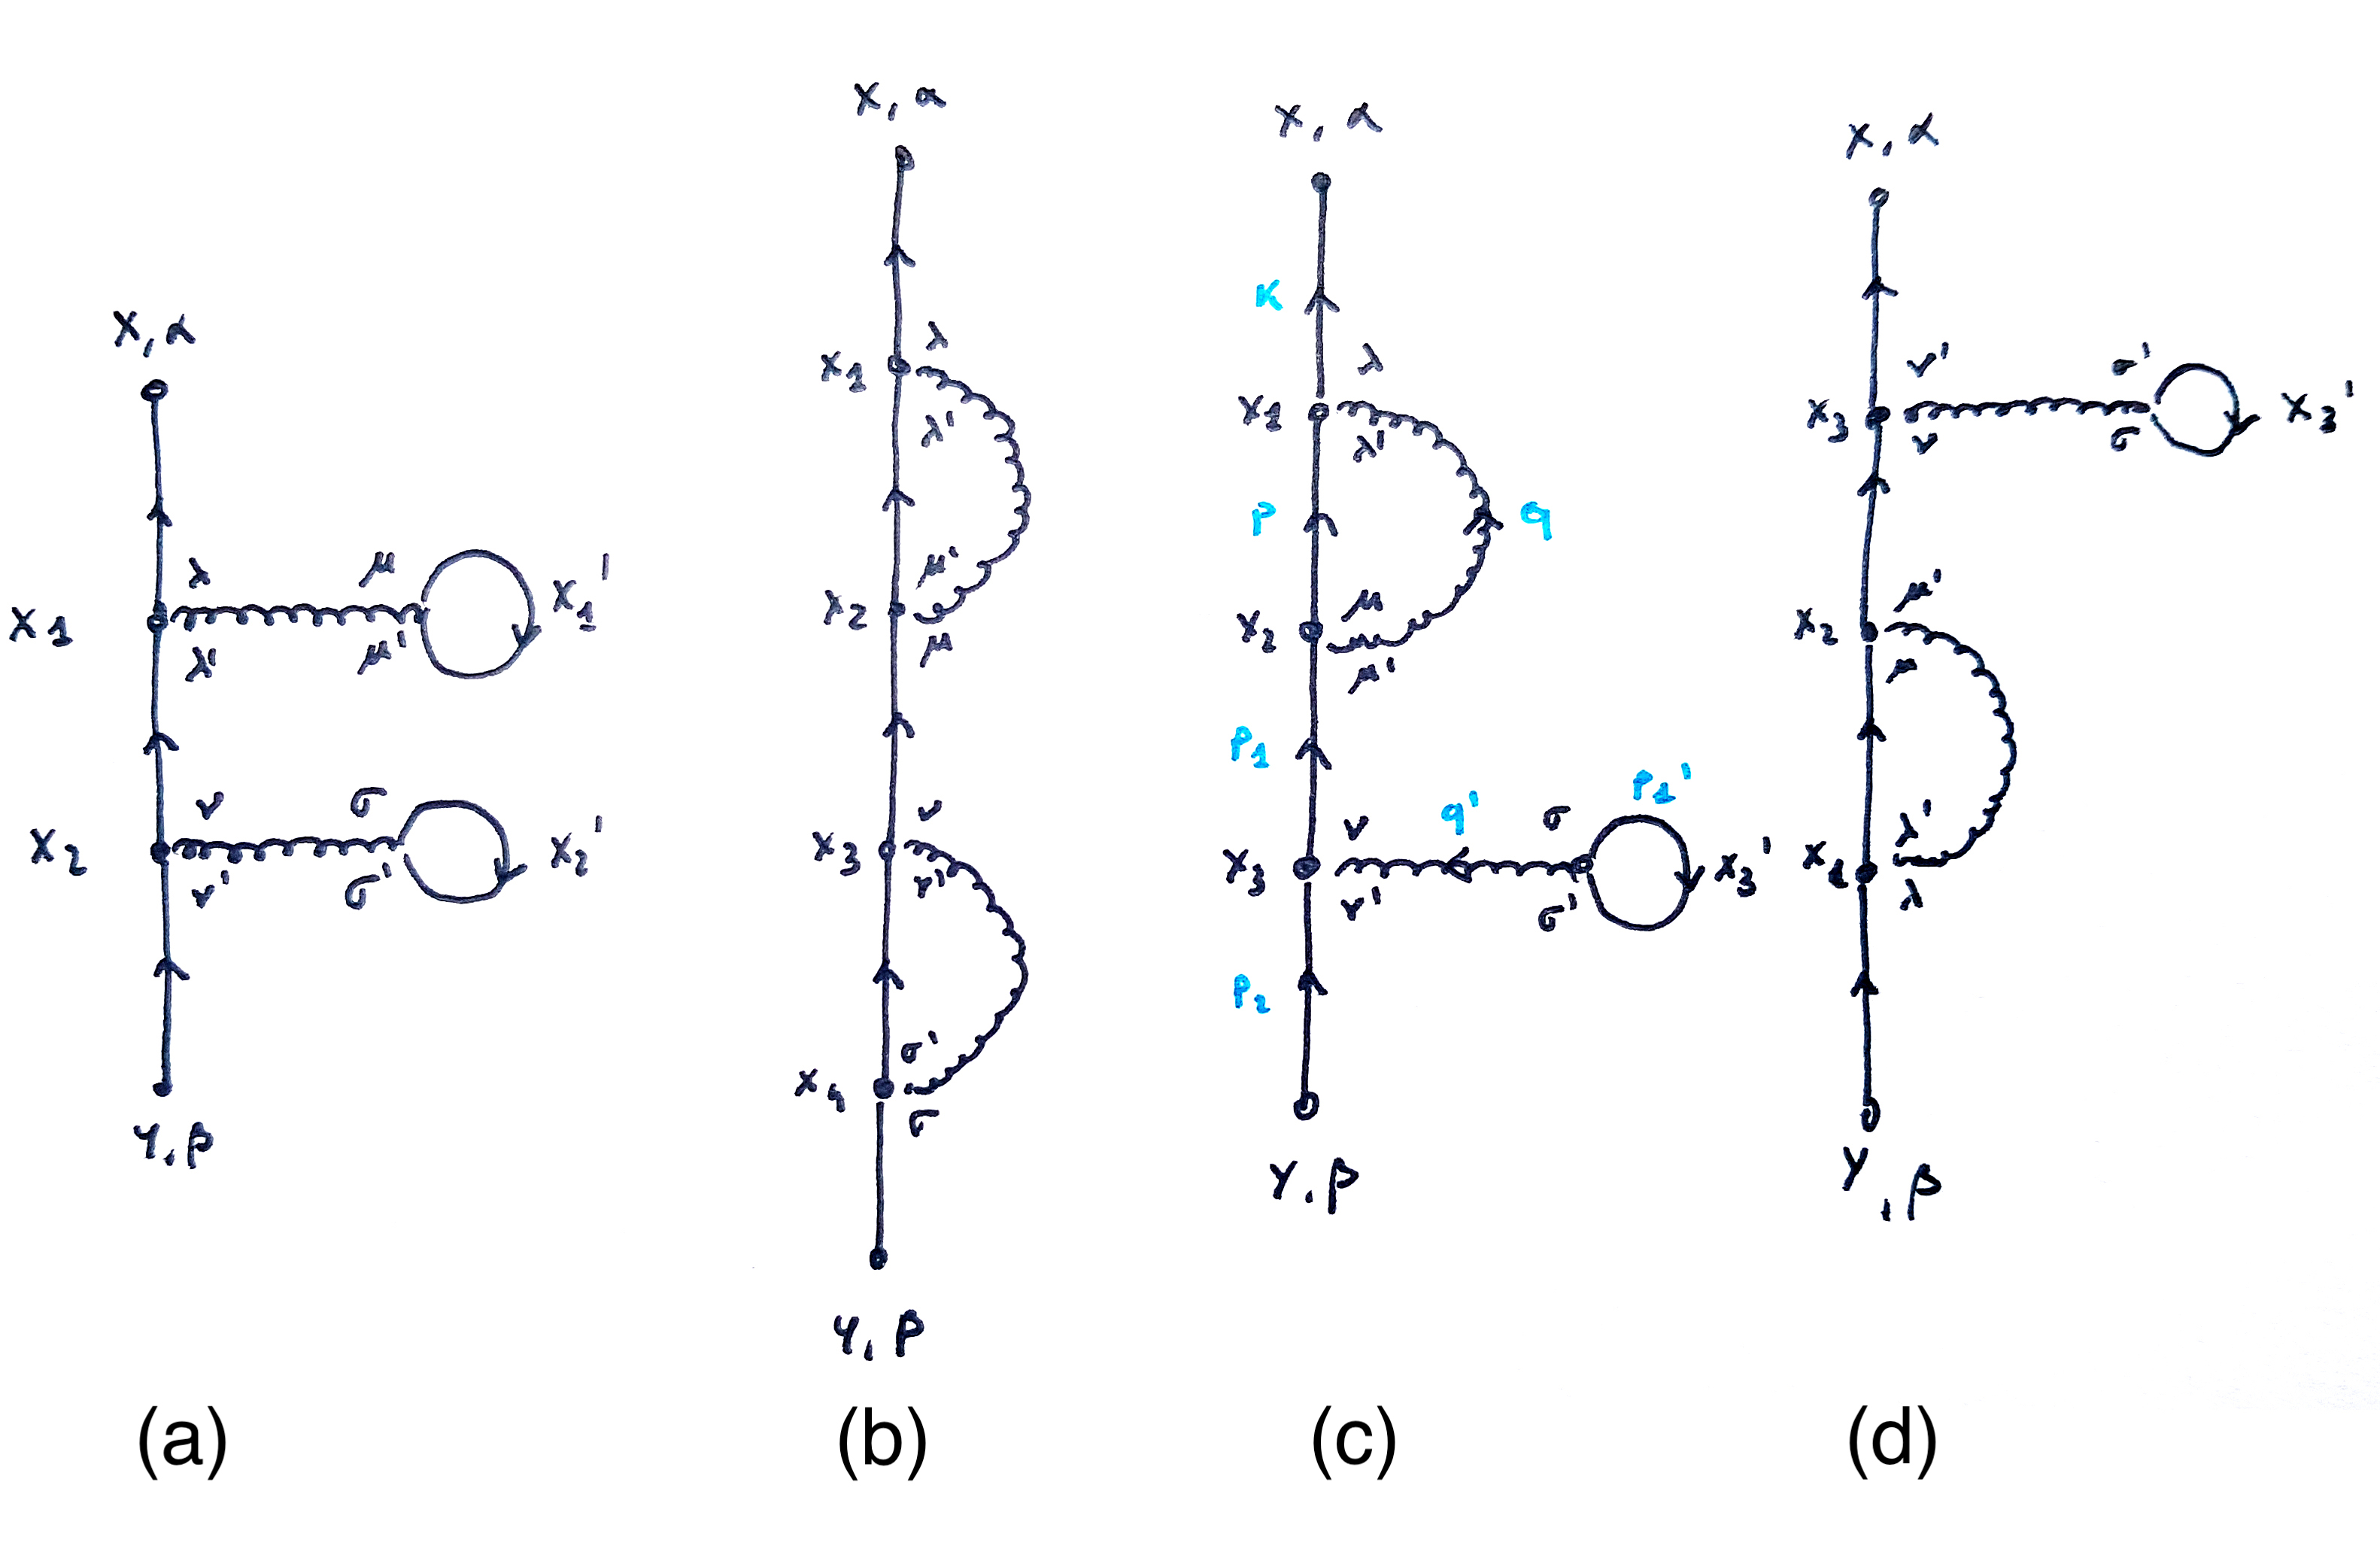
\includegraphics[width=\textwidth]{Diagrams1_1.jpg}
\end{figure}

\section*{Exercise (b)}

The $(c)$ and $(d)$ diagrams differ for the propagation direction of the particle.
Looking at their expression, we observe that:
\begin{equation*}
G^{(2c)}_{\alpha\beta}(x,y)  = G^{(2d)}_{\beta\alpha}(y,x)
\end{equation*}
which means they are equal unless a discrete parity transofmation that
\begin{align*}
(\alpha\beta)\rightarrow (\beta\alpha);\qquad (x,y)\rightarrow (y,x). 
\end{align*}
To state that two diagrams are topologically equivalent we must find a continuous transformation connecting the two, but this is not the case for diagrams $(c)$ and $(d)$ and thus they are distinct.

\section*{Exercise (c)}



The analitic expression of $G^{(2c)}_{\alpha\beta}(k)$ is given by the fourier transform:
\begin{align*}
G^{(2c)}_{\alpha\beta}(x,y) &=  \frac{1}{\hbar^2(2\pi)^{28}}\int \dd[4]{x_1}\dd[4]{x_2}\dd[4]{x_3}\dd[4]{x_3'}\int \dd[4]{k}\dd[4]{p}\dd[4]{q}\dd[4]{p_1}\dd[4]{q'}\dd[4]{p_1'}\dd[4]{p_2} \times \\
&\quad \times G^0_{\alpha\lambda}(k) V(\vb{q})_{\substack{\lambda\lambda' \\ \mu\mu'}}e^{i\omega_1 \eta} G^0_{\lambda'\mu'}(p) G^0_{\mu\nu}(p_1) V(\vb{q}')_{\substack{\nu\nu'\\ \sigma\sigma'}}e^{i\omega_2 \xi} G^0_{\sigma\sigma'}(p_1')G^0_{\nu'\beta}(p_2) \times \\
&\quad \times e^{ik(x-x_1)}e^{iq(x_1-x_2)}e^{ip(x_1-x_2)}e^{ip_1(x_2-x_3)}e^{iq'(x_3-x_3')}e^{ip_2(x_3-y)}
\end{align*}
rearranging the exponents of the exponential factors we recognize the Fourier expression for the following four-dimensional Dirac's deltas:
\begin{equation*}
\delta(p+q-k)\delta(p_1-q-p)\delta(q'+p_2-p_1)\delta(q')
\end{equation*}
which express the momentum conservation at each node of the diagram.
Once we substituted the previous expression into the Fourier transform, we exploit the integration over the internal variables, obtaining their elimination according to the arguments of the deltas:
\begin{align*}
G^{(2c)}_{\alpha\beta}(x,y) = \frac{1}{2\pi}\int \dd[4]{k}\frac{1}{\hbar^2(2\pi)^8} G^0_{\alpha\lambda}(k)\int \dd[4]{p} \dd[4]{p_1'}& V(\vb{k}-\vb{p})_{\substack{\lambda\lambda'\\ \mu\mu'}}e^{i\omega_{\vb{k}-\vb{p}} \eta}G^0_{\lambda'\mu'}(p) G^0_{\mu\nu}(k) \times \\
&\quad \times V(\vb{0})_{\substack{\nu\nu'\\ \sigma\sigma'}}e^{i\omega_{\vb{0}}\xi}G^0_{\sigma\sigma'}(P_1')G^0_{\nu'\beta}(k)
\end{align*}
hence the expression of the $(c)$ diagram in momentum space is:
\begin{equation*}
G^{(2c)}_{\alpha\beta}(k) = \frac{1}{\hbar^2(2\pi)^8} G^0_{\alpha\lambda}(k)\int \dd[4]{p} \dd[4]{p_1'}V(\vb{k}-\vb{p})_{\substack{\lambda\lambda'\\ \mu\mu'}}e^{i\omega_{\vb{k}-\vb{p}} \eta}G^0_{\lambda'\mu'}(p) G^0_{\mu\nu}(k) V(\vb{0})_{\substack{\nu\nu'\\ \sigma\sigma'}}e^{i\omega_{\vb{0}}\xi}G^0_{\sigma\sigma'}(P_1')G^0_{\nu'\beta}(k)
\end{equation*}
which can be rewritten restoring the four-dimensional notation as:
\begin{equation*}
G^{(2c)}_{\alpha\beta}(k) =  \frac{1}{\hbar^2(2\pi)^8} G^0_{\alpha\lambda}(k)\int \dd[4]{p} \dd[4]{p_1'} U(k-p)_{\substack{\lambda\lambda' \\ \mu\mu'}} G^0_{\lambda'\mu'}(p) G^0_{\mu\nu}(k)U(0)_{\substack{\nu\nu' \\ \sigma\sigma'}} G^0_{\sigma\sigma'}(p_1')G^0_{\nu'\beta}(k)e^{i\omega_{\vb{k}-\vb{p}} \eta}e^{i\omega_{\vb{0}}\xi}
 \end{equation*}
Remembering the fact that each non-interacting Green's function is diagonal in spin space and that we are considering spin-independent iteractions, we can factorize the spin part of the previous expression as:
\begin{align*}
S_{\alpha\beta} &= \delta_{\alpha\lambda} \delta_{\lambda\lambda'}\delta_{\mu\mu'}\delta_{\lambda'\mu'}\delta_{\mu\nu}\delta_{\nu\nu'}\delta_{\sigma\sigma'}\delta_{\sigma\sigma'}\delta_{\nu'\beta}\\
& = (2s+1)\delta_{\alpha\beta}
\end{align*}
thus we obtain:
\begin{equation*}
G^{(2c)}_{\alpha\beta}(k) =  \delta_{\alpha\beta}\frac{(2s+1)}{\hbar^2(2\pi)^8} G^0(k)\int \dd[4]{p} \dd[4]{p_1'} U(k-p)G^0_{\lambda'\mu'}(p) G^0(k)U(0)G^0(p_1')G^0(k)e^{i\omega_{\vb{k}-\vb{p}} \eta}e^{i\omega_{\vb{0}}\xi}.
 \end{equation*}



\end{document}


































